\documentclass[../thesis.tex]{subfiles}

% \usepackage{booktabs}
% \usepackage{subcaption}
% \usepackage{graphicx}
% \usepackage{multirow}
% \usepackage{caption}
% %\usepackage{minipage}
% \usepackage{amsmath,amssymb}
% \usepackage{lib}
% \usepackage{multicol}
% \usepackage{epstopdf}
% \usepackage[pagebackref=true,breaklinks=true,letterpaper=true,colorlinks,bookmarks=false]{hyperref}

% \usepackage{balance}

% \let\svthefootnote\thefootnote
% \newcommand\blfootnote[1]{%
% \begingroup
% \let\thefootnote\relax\footnote{#1}
% \addtocounter{footnote}{-1}\let\thefootnote\svthefootnote
% \endgroup
% }




% cite.sty was written by Donald Arseneau
% V1.6 and later of IEEEtran pre-defines the format of the cite.sty package
% \cite{} output to follow that of the IEEE. Loading the cite package will
% result in citation numbers being automatically sorted and properly
% "compressed/ranged". e.g., [1], [9], [2], [7], [5], [6] without using
% cite.sty will become [1], [2], [5]--[7], [9] using cite.sty. cite.sty's
% \cite will automatically add leading space, if needed. Use cite.sty's
% noadjust option (cite.sty V3.8 and later) if you want to turn this off
% such as if a citation ever needs to be enclosed in parenthesis.
% cite.sty is already installed on most LaTeX systems. Be sure and use
% version 5.0 (2009-03-20) and later if using hyperref.sty.
% The latest version can be obtained at:
% http://www.ctan.org/pkg/cite
% The documentation is contained in the cite.sty file itself.
%
% Note that some packages require special options to format as the Computer
% Society requires. In particular, Computer Society  papers do not use
% compressed citation ranges as is done in typical IEEE papers
% (e.g., [1]-[4]). Instead, they list every citation separately in order
% (e.g., [1], [2], [3], [4]). To get the latter we need to load the cite
% package with the nocompress option which is supported by cite.sty v4.0
% and later. Note also the use of a CLASSOPTION conditional provided by
% IEEEtran.cls V1.7 and later.

% \hyphenation{op-tical net-works semi-conduc-tor}


\begin{document}


Consider the chairs in \figref{fig1_cat}. As humans, not only can we infer at a glance that the image contains three chairs, we also construct a rich internal representation of each of them such as their locations and 3D poses. Moreover, we have a guess of their 3D shapes, even though we might never have seen these particular chairs. We can do this because we do not experience this image {\em tabula rasa}, but in the context of our  ``remembrance of things past".   Previously seen chairs enable us to develop a notion of the 3D shape of chairs, which we can project to the instances in this particular image. We also specialize our representation to these particular instances (e.g. any custom decorations they might have), signalling that both top-down and bottom-up cues influence our percept~\cite{nandakumar2011little}. In this chapter, we incorporate these principles in a computational framewoek for reconstructing objects given a single image. 

The task of reconstructing objects from a single image is a challenging one -- a typical image depicts many objects, each possibly belonging to a different object category; an object category, in turn, comprises instances of varying shapes, textures, size \etc and any particular instance may be viewed from a different viewpoint. Previous approaches to this problem can be broadly grouped into two paradigms. The paradigm of model-based object reconstruction has reflected varying preferences on model representations.  Generalized cylinders~\cite{nevatia1977description} resulted in very compact descriptions for certain classes of shapes, and can be used for category level descriptions, but the fitting problem for general shapes is challenging. Polyhedral models~\cite{gupta2010blocks,xiao2012localizing}, which trace back to the early work of Roberts \cite{roberts1963machine}, and CAD models~\cite{limparsing,satkin20143dnn,Pepik_2015_CVPR_Workshops}, cannot perfectly deform into shapes even slightly different from those in training data, but given a set of point correspondences can be quite effective for determining approximate instance viewpoints. Some recent methods have proposed using similar instances from a collection of CAD models \cite{su2014estimating,huang2015single} for  non-parametric reconstruction but their applications have been restricted to pre-segmented online product images or recovering 3D from 2.5D object scans~\cite{sung2015data}. Here we pursue more expressive basis shape models~\cite{Anguelov:SCAPE2005,blanz1999morphable,zia2013detailed} which establish a balance between the two extremes as they can deform but only along class-specific modes of variation.

\begin{figure}[t]
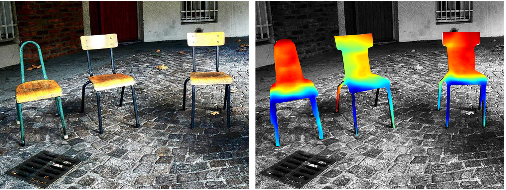
\includegraphics[width = \textwidth]{figures/categoryshapes/teaserChair.pdf}
\caption{Example outputs of our system, given a single image of a scene having chairs, a class that the system was exposed to during training. The coloring on the right image signals object-centric depth (we do not aim for globally consistent depths across multiple objects). Blue means close to the camera, red means far from the camera.}
  \figlabel{fig1_cat}
\end{figure}

The alternate paradigm comprises of approaches that target the problem of object reconstruction in a class or object agnostic manner, either implicitly or explicitly using generic learned 3D shape cues \cite{hoiem2005automatic, saxena2009make3d}, or bottom-up cues and the physics of image formation \cite{Karsch2013,barronPAMI13} building upon the long tradition of Shape-from-X, which traces back to seminal work by Horn \cite{HORNThesis1970}. These methods, while quite general, have not yet been demonstrated for 3D reconstruction -- as opposed to 2.5D -- and typically assume known object segmentation \cite{barronPAMI13}. Some recent approaches have demonstrated the use of supervised learning techniques to implcitly learn generic cues to predict depth maps \cite{eigennips14} and surface normals \cite{eigen2015predicting, wang2015designing} but these have primarily focused on  inferring scene-level information which differs from our goal of perceiving the shape of objects.

In this chapter, we combine both these reconstruction paradigms - we obtain top-down shape information from our model-based reconstruction approach and complement it with bottom-up shape information obtained via an intrinsic image decomposition method.  Crucially, in contrast to previous work (e.g. \cite{barronPAMI13,carvi14,cashman2013dolphins}), we do not require perfect knowledge of object localization and pose as our reconstruction is driven by automatic figure-ground object segmentations and viewpoint estimations.

\begin{figure}[t]
\centering
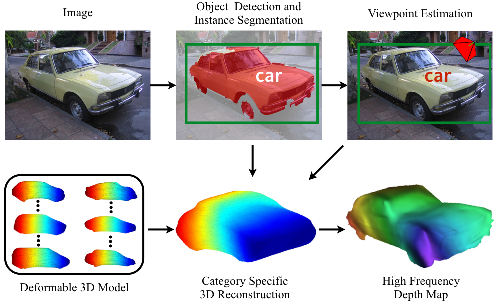
\includegraphics[width = .9\textwidth]{figures/categoryshapes/figTest.pdf}
\caption{Overview of our full reconstruction method. We leverage estimated instance segmentations and predicted viewpoints to generate a full 3D mesh and a high frequency 2.5D depth map for each object in the image.}
\figlabel{figTest}
\end{figure}

The framework we propose to reconstruct the objects present in an image is outlined in \figref{figTest}. As a first step, we leverage the recent progress made by the computer vision community in object detection~\cite{girshick2013rich} and instance segmentation~\cite{BharathECCV2014, BharathCVPR2015} to identify and localize objects in the image. For each object, we also predict a viewpoint in the form of three euler angles. We then use our learned deformable 3D shape models in conjunction with the viewpoint and localization information to produce a ``top-down'' 3D reconstruction for the object guided primarily by category level cues. Finally, we infuse our 3D shape with high frequency local shape cues to obtain our end result - a rich 3D reconstruction of the object. We briefly outline each of the components required for the above proposed framework.

\paragraph{Learning Deformable 3D Models.}
As noted earlier, previously seen objects allow us to develop a notion of 3D shape which informs inference for new instances. We present an algorithm that can build category-specific  deformable shape models from just images with 2D annotations (segmentation masks and a small set of keypoints) present in modern computer vision datasets (e.g. PASCAL VOC~\cite{pascal-voc-2012}). These learnt shape models and deformations allow us to robustly infer shape while capturing intra-class shape variation.

% \paragraph{Learning to Estimate Viewpoint.}
% The first step towards being able to represent objects in 3D is to predict their viewpoint. This intermediate representation provides coarse information about the shape and its inference is a well studied problem in computer vision \cite{huttenlocher1990recognizing, rothganger20063d, gordon2006and, savarese2008view, xiao2008structuring, gu2010discriminative, ozuysal2009pose}.
% We train a Convolutional Neural Network (CNN) ~\cite{neocognitron,LeCun1989} based architecture which can implicitly capture and aggregate local evidence to obtain a viewpoint estimate and demonstrate improvements over the state-of-the-art for this task.

\paragraph{Object Shape Recovery.}
Given an object's category, approximate localization and viewpoint, we obtain a 3D reconstruction for the corresponding object using the learned category-specific deformable shape model. We complement the top-down shape inferred via this inference with a bottom-up module that further refines our shape estimate for a particular instance. This framework allows us to capture the coarse as well as fine level shape details for objects from a single image.

This chapter is organized as follows: in \secref{modelLearning} we describe our model learning pipeline where we estimate camera parameters for all training objects (\secref{nrsfm}) followed by our shape model formulation (\secref{basisshapes}) to learn 3D models. \secref{testing} describes our testing pipeline where we leverage our learnt models alongwith object recognition systems (detection~\cite{girshick2013rich}, segmentation~\cite{BharathCVPR2015}, pose estimation~\cite{ShubhamPose}) to reconstruct novel instances without assuming any annotations. We quantitatively evaluate the various components of our approach in \secref{experiments} and provide sample reconstructions in the wild.

% This journal paper extends our earlier work~\cite{categoryShapesKar15} by providing a detailed exposition of our viewpoint prediction system and its systematic evaluation previously presented in \cite{ShubhamPose}. We also report updated experiments with a slightly modified mesh metric and using improved versions of our pose prediction~\cite{ShubhamPose} and instance segmentation~\cite{BharathCVPR2015} systems.

\section{Learning Deformable 3D Models}
\seclabel{modelLearning}

\begin{figure*}[htb!]
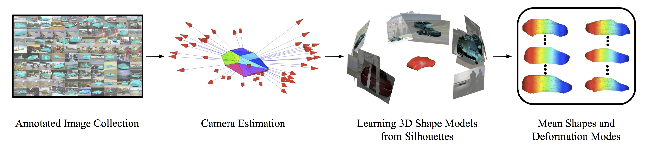
\includegraphics[width = \textwidth]{figures/categoryshapes/figTrain.pdf}
\caption{Overview of our training pipeline. We use an annotated image collection to estimate camera projection parameters which we then use along with object silhouettes to learn 3D shape models. Our learnt shape models, as illustrated in the rightmost figure are capable of deforming to capture intra-class shape variation.}
\label{fig:figtrain}
\end{figure*}

We are interested in learning 3D shape models that can be robustly aligned to noisy object segmentations by incorporating top-down class-specific knowledge of how shapes from the class typically project onto the image. We want to learn such models from just 2D training images, aided by ground truth segmentations and a few keypoints, similar to \cite{carvi14}. Our approach operates by first estimating the projection parameters (camera) for all objects in a class using a structure-from-motion approach, followed by optimizing over a deformation basis of representative 3D shapes that best explain all silhouettes, conditioned on the estimated cameras. We describe these two stages of model learning in the following subsections. Figure \ref{fig:figtrain} illustrates this training pipeline of ours.

\subsection{Camera Estimation}
\seclabel{nrsfm}
We use the framework of NRSfM \cite{Bregler2000} to jointly estimate the projection parameters (rotation, translation and scale) for all training instances in each class. Originally proposed for recovering shape and deformations from video \cite{nrsfm_priors,Torresani2008NRSFM,varnrsfm2013,Bregler2000}, NRSfM is a natural choice for camera estimation from sparse correspondences as intra-class variation may become a confounding factor if not modeled explicitly. However, the performance of such algorithms has only been explored on simple categories, such as SUV's \cite{Zhu_ModelEvolution:2010} or flower petal and clown fish \cite{prasad2010finding}. Closer to our work, Hejrati and Ramanan \cite{HejratiR12} used NRSfM on a larger class (cars) but need a predictive detector to fill-in missing data (occluded keypoints) which we do not assume to have here.

%To cope with the highly under-constrained nature of the problem most methods have dwelled on low-rank factorizations of the shape matrix \cite{Bregler2000,Brand2005}, or on imposing priors on shapes and deformations \cite{Torresani2008NRSFM,nrsfm_priors,varnrsfm2013}. }

We closely follow the EM-PPCA formulation of Torresani \etal\cite{Torresani2008NRSFM} and propose a simple extension to the algorithm that incorporates silhouette information in addition to keypoint correspondences to robustly recover cameras and shape bases. Energies similar to ours have been proposed in the shape-from-silhouette  \cite{balloonshapes} and rigid structure-from-motion \cite{carvi14} literature but, to the best of our knowledge, not in conjunction with NRSfM.

\vspace{3mm}
\noindent \textbf{NRSfM Model Formulation.} We are provided with an annotated training set $T:\{(O_n, P_n)\}_{n=1}^N$, where $O_n$ is the instance silhouette and $P_n \in \mathbb{R}^{2 \times K}$ denotes the annotated keypoint coordinates, possibly with missing entries (occluded/truncated keypoints). The annotated keypoints $P_n$ are  projections of the underlying 3D points $W_n \in \mathbb{R}^{3 \times K}$ via the projection function $\pi_n$. In the \nrsfm model, the space of 3D keypoint locations $W_n$ is parametrized linearly and the projection function is assumed to be weakly orthographic \ie $\pi_n \equiv (c_n, R_n, T_n)$, where $c_n$ represents scale, $R_n \in \mathbb{R}^{2 \times 3}$ denotes rotation and $T_n \in \mathbb{R}^{1 \times 2}$ corresponds to 2D translation. Our goal is to infer the camera parameters $(c_n, R_n, T_n)$ as well as 3D keypoint locations $W_n$ for all instances in the annotated training set.

Formally, our adaptation of the \nrsfm algorithm in \cite{Torresani2008NRSFM} corresponds to maximizing the likelihood of the following model:

\begin{equation}
\begin{aligned}
&{P_{n}} = c_nR_nW_{n} + 1^TT_{n} + N_{n}\\
&W_n = \bar{W} + \sum\limits_{k=1}^B U_b z_{nb} \\
&z_n \sim \mathcal{N}(0,I), \quad N^k_{n}\sim \mathcal{N}(0,\sigma^2 I)
\end{aligned}
\end{equation}
\begin{align}
\text{subject to:}\nonumber &\quad R_nR_{n}^{T} = I_2 \\
%\quad \forall n\in \{1,\cdots,N\}
\eqlabel{sil_constraint}
\sum\limits_{k=1}^K C_{n}^{mask}(p_{k,n}) &= 0, \quad \forall n\in \{1,\cdots,N\}
\end{align}

Here, the (partially) observed keypoint locations $P_n$ are assumed to be the projection under $\pi_n \equiv (c_n, R_n, T_n)$ of the 3D shape $W_n$ with white noise $N_n$. The shape is parameterized as a factored Gaussian with a mean shape $\bar{W}$, $B$ basis vectors $[U_1,U_2, \cdots,U_B] = U$ and latent deformation parameters $z_n$. Our key modification is constraint in \eqref{sil_constraint} where $C_{n}^{mask}$ denotes the Chamfer distance field of the $n^{th}$ instance's binary mask and says that all keypoints $p_{k,n}$ of instance $n$ should lie inside its binary mask. We observed that this results in more accurate cameras as well as more meaningful shape bases learnt from the data.

\vspace{3mm}
\noindent \textbf{Learning.} The likelihood of the above model is maximized using the EM algorithm. Missing data (occluded keypoints) is dealt with by ``filling-in" the values using the forward equations after the E-step. The algorithm computes shape parameters $\{\bar{W},U\}$, rigid body transformations $\{c_n,R_n,T_n\}$ as well as the deformation parameters $\{z_n\}$ for each training instance $n$. In practice, we augment the data using horizontally mirrored images to exploit bilateral symmetry in the object classes considered. We also precompute the Chamfer distance fields for the whole set to speed up computation. As shown in \figref{nrsfm_images}, \nrsfm  allows us to reliably predict cameras while being robust to intraclass variations.

\begin{figure}[htb!]
  \centering
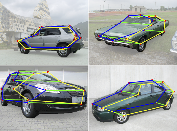
\includegraphics[width=.8\linewidth]{figures/categoryshapes/NRSFMCars.pdf}
\caption{NRSfM camera estimation: Estimated cameras visualized using a 3D car wireframe.}
\figlabel{nrsfm_images}
\end{figure}


\subsection{3D Basis Shape Model Learning}
\seclabel{basisshapes}
Equipped with camera projection parameters and keypoint correspondences (lifted to 3D by NRSfM) on the whole training set, we proceed to build deformable 3D shape models from object silhouettes within the same class. 3D shape reconstruction from multiple silhouettes projected from a single object in calibrated settings has been widely studied. Two prominent approaches are \textit{visual hulls} \cite{laurentini1994hull} and variational methods derived from \textit{snakes} e.g \cite{esteban2004snake,yusuf2006snake} which deform a surface mesh iteratively until convergence. Some interesting recent papers have extended variational approaches to handle categories \cite{cashman2013dolphins,chen20123d} but typically require some form of 3D annotations to bootstrap models. A recently proposed visual-hull based approach \cite{carvi14} requires only 2D annotations as we do for class-based reconstruction and it was successfully demonstrated on PASCAL VOC but does not serve our purpose as it makes strong assumptions about the accuracy of the segmentation and will in fact fill entirely any segmentation with a voxel layer. In contrast, we build parametric shape models for categories that compactly capture intra class shape variations. The benefits of having a model of 3D shape are manifold: 1) we are more robust to noisy inputs (silhouettes and pose) allowing us to pursue reconstruction in a fully automatic setting and 2) we can potentially sample novel shapes from an object category.

%We propose an algorithm to learn class-specific 3D shape models given silhouette information and camera viewpoints estimated in the previous section. Our shape models inherently capture the intraclass variations in object categories and can be used to recover a 3D shape given an object's approximate silhouette and viewpoint in a new image.

\paragraph{Shape Model Formulation.} We model our category shapes as a deformable point cloud - one per object class. As in the \nrsfm model, we use a linear combination of basis vectors to model these deformations. Note that we learn such models from silhouettes and this is what enables us to learn deformable models without relying on point correspondences between scanned 3D exemplars~\cite{blanz2003face}.

%In order to capture the intra-class variations using a single shape model, we must incorporate possible deformations. Similar to the NRSfM approach, the deformations we allow are a linear combination of  deformation bases. This setup, while using a formulation similar to NRSfM is significantly different because we do not assume any known correspondences or annotated points across images and the shape models we aim to infer are much denser (because of the large number of points in the representation).

The annotated training set $T:\{(O_n, P_n)\}_{n=1}^N$, where $O_n$ is the instance silhouette and $P_n \in \mathbb{R}^{2 \times K}$ denotes the annotated keypoint coordinates, is augmented after \nrsfm to contain $\pi_n$ (the projection function from world to image coordinates) and $W_n$ (3D coordinates for a small set of keypoints).
Our shape model $M = (\overline{S},V)$ comprises of a mean shape $\overline{S}$ and deformation bases $V = \{ V_1,.,V_K \} $ learnt from the augmented training set $T:\{(O_n,\pi_n, W_n)\}_{n=1}^N$. Note that the $\pi_i$ we obtain using NRSfM corresponds to orthographic projection but our algorithm could handle perspective projection as well.

In addition to the above, we use the following notations  --  $\pi(S)$ corresponds to the 2D projection of shape $S$, $C^{mask}$ refers to the Chamfer distance field of the binary mask of silhouette $O$ and $\Delta^k(p;Q)$ is defined as the squared average distance of point $p$ to its $k$ nearest neighbors in set $Q$.

\paragraph{Energy Formulation.} We formulate our objective function primarily based on image silhouettes. For example, the shape for an instance should always project within its silhouette and should agree with the keypoints (lifted to 3D by \nrsfm). We capture these by defining corresponding energy terms as follows:


\paragraph{Silhouette Consistency.} Silhouette consistency simply enforces the predicted shape for an instance to project inside its silhouette. This can be achieved by penalizing the points projected outside the instance mask by their distance from the silhouette (\ie squared distance to the closest silhouette point). In our $\Delta$ notation it can be written as follows:
\begin{gather}
 \label{eq:sil_con}E_{s}(S,O,\pi)=\underset{C^{mask}(p)>0}{\sum}\Delta^1(p;O)
\end{gather}


\paragraph{Silhouette Coverage.}
Using silhouette consistency alone would just drive points projected outside in towards the silhouette. This wouldn't ensure though that the object silhouette is ``filled'' - i.e. there might be overcarving. We deal with it by having an energy term that encourages points on the silhouette to pull nearby projected points towards them. Formally, this can be expressed as:
\begin{gather}
    \label{eq:sil_cov}E_{c}(S,O,\pi)=\underset{p\in O}{\sum}\Delta^m(p;\pi(S))
\end{gather}


\paragraph{Keypoint Consistency.} Our \nrsfm algorithm provides us with sparse 3D keypoints along with camera projection parameters. We use these sparse correspondences on the training set to deform the shape to explain these 3D points. The corresponding energy term penalizes deviation of the shape from the 3D keypoints $W$ for each instance. Specifically, this can be written as:
\begin{gather}
    \label{eq:kpgrad}E_{kp}(S,W)=\underset{\kappa\in W}{\sum}\Delta^m(\kappa;S)
\end{gather}


\paragraph{Local Consistency.} In addition to the above data terms, we use a simple shape regularizer to restrict arbitrary deformations by imposing a quadratic deformation penalty between every point and its neighbors. We also impose a similar penalty on deformations to ensure local smoothness. The $\delta$ parameter represents the mean squared displacement between neighboring points and it encourages all faces to have similar size. Here $V_{ki}$ is the $i^{th}$ point in the $k^{th}$ basis.
\begin{gather}
 \label{eq:local_con}E_{l}(\bar{S},V)=\underset{i}{\sum}\underset{j\in N(i)}{\sum}((\|\bar{S}_{i}-\bar{S}_{j}\| - \delta)^2 + \underset{k}{\sum}\|V_{ki}-V_{kj}\|^2)
 \end{gather}
 

\paragraph{Normal Smoothness.} Shapes occurring in the natural world tend to be locally smooth. We capture this prior on shapes by placing a cost on the variation of normal directions in a local neighborhood in the shape. Our normal smoothness energy is formulated as
\begin{gather}
 \label{eq:normal_con}E_{n}(S)=\underset{i}{\sum}\underset{j\in N(i)}{\sum}(1-\vec{\mathcal{N}_i} \cdot \vec{\mathcal{N}_j})
\end{gather}
 Here, $\vec{\mathcal{N}_i}$ represents the normal for the $i^{th}$ point in shape $S$ which is computed by fitting planes to local point neighborhoods. Our prior essentially states that local point neighborhoods should be flat. Note that this, in conjunction with our previous energies automatically enforces the commonly used prior that normals should be perpendicular to the viewing direction at the occluding contour~\cite{Barron2012B}.

Our total energy is given in equation \eqref{formulation}. In addition to the above smoothness priors we also penalize the $L_2$ norm of the deformation parameters $\alpha_i$ to prevent unnaturally large deformations.
\begin{gather}
\eqlabel{formulation}
E_{tot}(\bar{S},V,\alpha) = E_{l}(\bar{S},V)+\underset{i}{\sum}(E_{s}^i+E_{kp}^i+E_{c}^i+E_{n}^i+\underset{k}{\sum}(\|\alpha_{ik}V_k\|_F^{2}))
\end{gather}


\paragraph{Learning.} We solve the optimization problem in equation~\eqref{optimization} to obtain our shape model $M=(\bar{S},V)$. The mean shape and deformation basis are inferred via block-coordinate descent on $(\bar{S},V)$ and $\alpha$ using sub-gradient computations over the training set. We restrict $\|V_k\|_F$ to be a constant to address the scale ambiguity between $V$ and $\alpha$ in our formulation. In order to deal with imperfect segmentations and wrongly estimated keypoints, we use truncated versions of the above energies that reduce the impact of outliers. The mean shapes learnt using our algorithm for 9 rigid categories in PASCAL VOC are shown in Figure \ref{fig:meanDense}. Note that in addition to representing the coarse shape details of a category, the model also learns finer structures like chair legs and bicycle handles, which become more prominent with deformations.

\begin{equation}
\begin{aligned}
\eqlabel{optimization}
& \underset{\bar{S},V,\alpha}{\text{min}}
& & E_{tot}(\bar{S},V,\alpha) \\
& \text{subject to:}
& & S^i = \bar{S} + \underset{k}{\sum}\alpha_{ik} V_k
\end{aligned}
\end{equation}

Our training objective is highly non-convex and  non-smooth and is susceptible to initialization. We follow the suggestion of \cite{esteban2004snake} and initialize our mean shape with a soft visual hull computed using all training instances. The deformation bases and deformation weights are initialized randomly. 


\paragraph{Implementation Details.}
The gradients involved in our optimization for shape and projection parameters are extremely efficient to compute. We use approximate nearest neighbors computed using k-d tree to implement silhouette coverage,  keypoint consistency gradients and leverage Chamfer distance fields for obtaining silhouette consistency gradients. Our overall computation takes only about 15 min to learn a deformable shape model for an object category with about 500 annotated examples.

\begin{figure}[htb!]
\centering
  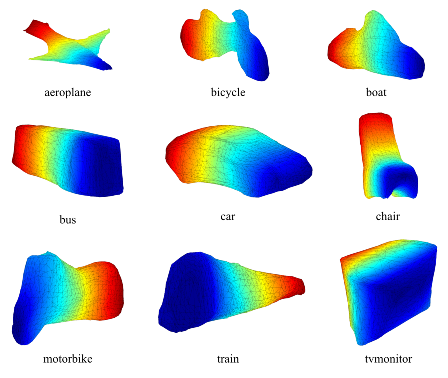
\includegraphics[width=\textwidth]{figures/categoryshapes/meanShapesCrop.pdf}
  \caption{Mean shapes learnt for rigid classes in PASCAL VOC obtained using our basis shape formulation. Color encodes depth when viewed frontally.}
  \label{fig:meanDense}
\end{figure}



\section{Learning to Predict Viewpoint}
\seclabel{viewpoints}

In our proposed framework, viewpoint prediction is an important component towards reconstructing the objects present in an image. We are interested in a system that is accurate across all instances of a category as well as robust to localization errors in object detection. We present a CNN based system for the viewpoint prediction task and demonstrate  that it leads to significant improvements over previous approaches.

\vspace{3mm}
\noindent \textbf{Related Work.}
Recently, CNNs have been shown to outperform Deformable Part Model (DPM) \cite{felzens_latent_pami10} based methods for recognition tasks \cite{rcnn,Krizhevsky}. Whereas DPMs explicitly model part appearances and their deformations, the CNN architecture allows such relations to be captured implicitly using a hierarchical convolutional structure.  Girshick \etal \cite{DPMsCNNs} argued that DPMs could also be thought as a specific instantiation of CNNs and therefore training an end-to-end CNN for the corresponding task should outperform a method which instead explicitly models part appearances and relations.

This result is particularly applicable to viewpoint estimation where the prominent approaches, from the initial instance based methods \cite{huttenlocher1990recognizing} to current state-of-the-art  \cite{pascal3d,pepik12dpm} explicitly model local appearances and aggregate evidence to infer viewpoint. Pepik \etal \cite{pepik12dpm} extend DPMs to 3D to model part appearances and rely on these to infer pose and Xiang \etal \cite{pascal3d} introduce a separate DPM component corresponding to each viewpoint. Ghodrati \etal \cite{ghodrati14viewpoint} differ from the explicit part-based methodology, using a fixed global descriptor to estimate viewpoint. We build on both these approaches by using a method which, while using a global descriptor, can implicitly capture part appearances.

\vspace{3mm}
\noindent \textbf{Formulation.}
We formulate the global pose estimation for rigid categories as predicting the viewpoint wrt to a canonical pose. This is equivalent to determining the three euler angles corresponding to azimuth ($\phi$), elevation($\varphi$) and cyclo-rotation($\psi$). We frame the task of predicting the euler angles as a classification problem where the classes $\{1,\ldots N_{\theta}\}$ correspond to $N_{\theta}$ disjoint angular bins. We note that the euler angles, and therefore every viewpoint, can be equivalently described by a rotation matrix. We will use the notion of viewpoints, euler angles and rotation matrices interchangeably.

\vspace{3mm}
\noindent \textbf{Learning.}
Viewpoint is manifested in a 2D image by the spatial relationships among the different features of the object. CNN based methods which can implicitly capture and hierarchically build on such relations are therefore suitable candidates for viewpoint prediction. Let $N_c$ be the number of object classes, $N_a$ be number of angles to be predicted per instance. The number of output units per class is $N_{a} \times N_{\theta}$ resulting in a total of $N_{c} \times N_{a} \times N_{\theta}$ outputs. We adopt an approach similar to Girshick \etal \cite{rcnn} and finetune a CNN model whose weights are initialized from a model pretrained on the Imagenet \cite{imagenet_cvpr09} classification task. We experimented with the architectures from Krizhevsky \etal \cite{Krizhevsky} (denoted as TNet) and Simonyan \etal \cite{Simonyan14c} (denoted as ONet). The architecture of our network is the same as the corresponding pre-trained network with an additional fully-connected layer having $N_{c} \times N_{a} \times N_{\theta}$ output units.

Instead of training a separate CNN for each class, we implement a loss layer that selectively considers the $N_{a} \times N_{\theta}$ outputs corresponding the class of the training instance and computes  a logistic loss for each of the angle predictions. This allows us to train a CNN which can jointly predict viewpoint for all classes, thus enabling learning a shared feature representation across all categories. We use the Caffe framework \cite{jia2014caffe} to train and extract features from the CNN described above. We also use data-augmentation by jittering ground-truth bounding boxes and generating additional training examples by using boxes that overlap with the annotated bounding box with IoU $>$ 0.7.


\section{Reconstruction in the Wild}
\seclabel{testing}
Given an image, our goal is to reconstruct the depicted objects. As the initial step, we use existing state-of-the-art systems~\cite{BharathECCV2014} to detect and segment the objects present in the image. We then proceed to individually reconstruct each of the detected objects. We approach the problem of reconstructing these objects from the big picture downward - like a sculptor first hammering out the big chunks and then chiseling out the details. We infer their coarse 3D poses and use these along with the predicted instance segmentations to fit our top-down shape models to obtain a coarse top-down shape (\secref{testingModel}). Finally, we recover high frequency shape details from shading cues present in the image (\secref{sirfs}).

\subsection{Category Specific Shape Inference}
\seclabel{testingModel}

We have at our disposal category-level deformable shape models which can be driven by data-specific and shape-prior based energy terms to infer an object's shape.  Recall that the proposed energy terms (\secref{basisshapes}), in particular silhouette consistency ($E_{s}(S,O,\pi)$) and silhouette coverage ($E_{c}(S,O,\pi)$) depend on a known object silhouette $O$ and camera projection $\pi$. We first describe how we estimate $O,\pi$ and then formulate an optimization  problem to infer object shape $S$.


\paragraph{Initialization.} Given an object detection along with its predicted instance segmentation, we use the largest connected component in the predicted segmentation to obtain the object silhouette $O$. We use the viewpoint prediction system described in \secref{viewpoints} to predict the viewpoint for the detected object, thereby obtaining the camera rotation $R$. Our learnt models are at a canonical bounding box scale - all objects are first resized to a particular width during training. Given the predicted bounding box, we scale the learnt mean shape accordingly and obtain camera scale $c$. The translation $T$ is initialized to be the center of the predicted bounding box. These provide us an initial estimate of the camera parameters $\pi_0 \equiv (c,R,T)$.


\paragraph{Formulation.}
We want to infer a shape that best explains the observed object silhouette, respects generic shape priors (smoothness, continuity) and lies on the linear manifold of category-level shapes. Note that, unlike model learning phase, we do not have access to annotated keypoint locations and thus do not enforce the reconstruction to explain any keypoint locations. These observations are incorporated by the reconstruction energy defined in \eqlabel{testRecon} (using $E_{s},E_{c},E_{n}$ defined in \secref{basisshapes}).

\begin{gather}
 \eqlabel{testRecon}E_{r} = E_{s} + E_{c} + E_{n}
\end{gather}

In addition to inferring the instance shape, we also observe that the initial camera estimate $\pi_0$ is only approximate as the $R$ is predicted upto a dicretization and $c,T$ are initialized coarsely. To alleviate this, we treat the camera parameters $\pi$ as optimization variables.  We further add regularizers to enforce the prior that shape deformation should be small and the the estimated camera should not deviate significantly from the initial camera estimate $\pi_0$ . Our final optimization for inferring the object reconstruction is given in \eqref{energyTest}.

\begin{equation}
\begin{aligned}
\eqlabel{energyTest}
& \underset{\alpha,\pi}{\text{min}}
& & E_{r}(S,\pi) + \delta(\pi,\pi_0) +\underset{k}{\sum}(\|\alpha_{k}V_k\|_F^{2})) \\
& \text{subject to:}
& & S = \bar{S} + \underset{k}{\sum}\alpha_{k} V_k
\end{aligned}
\end{equation}

\paragraph{Inference.} In the above optimization,  we first set the optimization variables $\alpha$ and $\pi$ to $0$ and $\pi_0$ respectively.  We then solve the above minimization for the deformation weights $\alpha$ as well as all the camera projection parameters $\pi$ (scale, translation and rotation) by optimizing~\eqref{optimization}  using block-coordinate descent (alternately optimizing $\pi$ and $\alpha$). The resulting output from the minimization provides us the projection parameters $\pi$ as well as the inferred 3D shape $S = \bar{S} + {\sum_k}\alpha_{k} V_k$. We use the efficient implementations of energy gradients described earlier and consequently, our overall computation takes only about 2 sec to reconstruct a novel instance using a single CPU core.

\renewcommand{\arraystretch}{1.4} 
\setlength{\tabcolsep}{8pt}
\begin{table*}
\centering
\footnotesize
\resizebox{1.0\linewidth}{!}{
\begin{tabular}{cccccccccccc|c}
\toprule 
	& 	& \textbf{aero}	& \textbf{bike}	& \textbf{boat}	& \textbf{bus}	& \textbf{car}	& \textbf{chair}	& \textbf{mbike}	& \textbf{sofa}	& \textbf{train}	& \textbf{tv}	& \textbf{mean}
\\
\midrule

\multirow{3}{*}{\textbf{Mesh}} 	& Ours	& \textbf{1.72} & \textbf{1.78} & 3.01 & \textbf{1.90} & 1.77 & \textbf{2.18} & 1.88 & \textbf{2.13} & \textbf{2.39} & \textbf{3.28} & \textbf{2.20} \\
& Carvi~\cite{carvi14}	& 1.87 & 1.87 & \textbf{2.51} & 2.36 & \textbf{1.41} & 2.42 & \textbf{1.82} & 2.31 & 3.10 & 3.39 & 2.31 \\
& Puff~\cite{twarog2012playing}	& 3.30 & 2.52 & 2.90 & 3.32 & 2.82 & 3.09 & 2.58 & 2.53 & 3.92 & 3.31 & 3.03 \\
\midrule
\multirow{3}{*}{\textbf{Depth}}	& Ours	& \textbf{9.51} & \textbf{9.27} & 17.20 & \textbf{12.71} & 9.94 & \textbf{7.78} & 9.61 & \textbf{13.70} & 31.58 & 8.78 & \textbf{13.01} \\
& Carvi~\cite{carvi14}	& 10.05 & 9.28 & \textbf{15.06} & 18.51 & \textbf{8.14} & 7.98 & \textbf{9.38} & 13.71 & \textbf{31.25} & \textbf{8.33} & 13.17 \\
& SIRFS~\cite{barronPAMI13}	& 13.52 & 13.79 & 20.78 & 29.93 & 22.48 & 18.59 & 16.80 & 18.28 & 40.56 & 20.18 & 21.49 \\
\bottomrule
\end{tabular}}
\caption{Studying the quality of our learnt 3D models: comparison between our method and \cite{carvi14,twarog2012playing} using ground truth keypoints and masks on PASCAL VOC.}
\label{tab:carvi_compare}
\end{table*}

\subsection{Bottom-up Shape Refinement}
\seclabel{sirfs}
The above optimization results in a top-down 3D reconstruction based on the category-level models, inferred object silhouette, viewpoint and our shape priors. We propose an additional processing step to recover high frequency shape information by adapting the intrinsic images algorithm of Barron and Malik \cite{barronPAMI13,Barron2012B}, SIRFS, which exploits statistical regularities between shapes, reflectance and illumination 
%For example, shapes are usually piecewise smooth and certain colors are more frequent than others. Bottom-up reconstruction approaches such as SIRFS are fundamentally more competent at estimating high frequency shape (e.g. door handles and lights in cars), which vary considerably between different object instances, but have trouble capturing rough global shape, which is more stable across a class and is characterized by long-range dependencies.
Formally, SIRFS is formulated as the following optimization problem:
\begin{equation}
\begin{aligned}
& \underset{Z,L}{\text{minimize}}
& & g(I-S(Z,L))+f(Z)+h(L)
\end{aligned}
\end{equation}
where $R=I-S(Z,L)$ is a log-reflectance image, $Z$ is a depth map and $L$ is a spherical-harmonic model of illumination. $S(Z,L)$ is a rendering engine which produces a log shading image with the illumination $L$. $g$, $f$ and $h$ are the loss functions corresponding to reflectance, shape and illumination respectively.

%A recent paper \cite{Karsch2013} showed that even human-provided annotation of the curvature at internal object contours is insufficient for reliable global shape estimation. Here we instead opt to compute coarse shape top-down and incorporate it into the optimization using an extended version of SIRFS. The loss term we use to this effect is as follows:
We incorporate our current coarse estimate of shape into SIRFS through an additional loss term:

\begin{equation}
f_o(Z,Z') = \underset{i}{\sum}((Z_i-Z_i')^2+\epsilon^2)^{\gamma_o}
\end{equation}
where $Z'$ is the initial coarse shape and $\epsilon$ a parameter added to make the loss differentiable everywhere. We obtain $Z'$ for an object by rendering a depth map of our fitted 3D shape model which guides the optimization of this highly non-convex cost function. The outputs from this bottom-up refinement are reflectance, shape and illumination maps of which we retain the shape.



\newcommand{\gtViewWidth}{0.15}
\newcommand{\gtViewFormat}{pdf}
\begin{figure*}[htb!]
\includegraphics[width=\gtViewWidth\textwidth]{figures/categoryshapes/predictionVisualizationsVgg/aeroplane/42.\gtViewFormat} \hfill
\includegraphics[width=\gtViewWidth\textwidth]{figures/categoryshapes/predictionVisualizationsVgg/aeroplane/85.\gtViewFormat}
\includegraphics[width=\gtViewWidth\textwidth]{figures/categoryshapes/predictionVisualizationsVgg/aeroplane/125.\gtViewFormat} \hfill
\includegraphics[width=\gtViewWidth\textwidth]{figures/categoryshapes/predictionVisualizationsVgg/aeroplane/166.\gtViewFormat} \hfill
\includegraphics[width=\gtViewWidth\textwidth]{figures/categoryshapes/predictionVisualizationsVgg/aeroplane/207.\gtViewFormat}
\includegraphics[width=\gtViewWidth\textwidth]{figures/categoryshapes/predictionVisualizationsVgg/aeroplane/251.\gtViewFormat}

\includegraphics[width=\gtViewWidth\textwidth]{figures/categoryshapes/predictionVisualizationsVgg/bicycle/20.\gtViewFormat} \hfill
\includegraphics[width=\gtViewWidth\textwidth]{figures/categoryshapes/predictionVisualizationsVgg/bicycle/36.\gtViewFormat} \hfill
\includegraphics[width=\gtViewWidth\textwidth]{figures/categoryshapes/predictionVisualizationsVgg/bicycle/57.\gtViewFormat}
\includegraphics[width=\gtViewWidth\textwidth]{figures/categoryshapes/predictionVisualizationsVgg/bicycle/78.\gtViewFormat} \hfill
\includegraphics[width=\gtViewWidth\textwidth]{figures/categoryshapes/predictionVisualizationsVgg/bicycle/95.\gtViewFormat} \hfill
\includegraphics[width=\gtViewWidth\textwidth]{figures/categoryshapes/predictionVisualizationsVgg/bicycle/114.\gtViewFormat}

\includegraphics[width=\gtViewWidth\textwidth]{figures/categoryshapes/predictionVisualizationsVgg/bus/22.\gtViewFormat} \hfill
\includegraphics[width=\gtViewWidth\textwidth]{figures/categoryshapes/predictionVisualizationsVgg/bus/49.\gtViewFormat} \hfill
\includegraphics[width=\gtViewWidth\textwidth]{figures/categoryshapes/predictionVisualizationsVgg/bus/70.\gtViewFormat}
\includegraphics[width=\gtViewWidth\textwidth]{figures/categoryshapes/predictionVisualizationsVgg/bus/98.\gtViewFormat} \hfill
\includegraphics[width=\gtViewWidth\textwidth]{figures/categoryshapes/predictionVisualizationsVgg/bus/120.\gtViewFormat} \hfill
\includegraphics[width=\gtViewWidth\textwidth]{figures/categoryshapes/predictionVisualizationsVgg/bus/142.\gtViewFormat}

\includegraphics[width=\gtViewWidth\textwidth]{figures/categoryshapes/predictionVisualizationsVgg/car/49.\gtViewFormat} \hfill
\includegraphics[width=\gtViewWidth\textwidth]{figures/categoryshapes/predictionVisualizationsVgg/car/92.\gtViewFormat} \hfill
\includegraphics[width=\gtViewWidth\textwidth]{figures/categoryshapes/predictionVisualizationsVgg/car/137.\gtViewFormat}
\includegraphics[width=\gtViewWidth\textwidth]{figures/categoryshapes/predictionVisualizationsVgg/car/186.\gtViewFormat} \hfill
\includegraphics[width=\gtViewWidth\textwidth]{figures/categoryshapes/predictionVisualizationsVgg/car/232.\gtViewFormat} \hfill
\includegraphics[width=\gtViewWidth\textwidth]{figures/categoryshapes/predictionVisualizationsVgg/car/279.\gtViewFormat}

\includegraphics[width=\gtViewWidth\textwidth]{figures/categoryshapes/predictionVisualizationsVgg/chair/36.\gtViewFormat} \hfill
\includegraphics[width=\gtViewWidth\textwidth]{figures/categoryshapes/predictionVisualizationsVgg/chair/73.\gtViewFormat} \hfill
\includegraphics[width=\gtViewWidth\textwidth]{figures/categoryshapes/predictionVisualizationsVgg/chair/112.\gtViewFormat}
\includegraphics[width=\gtViewWidth\textwidth]{figures/categoryshapes/predictionVisualizationsVgg/chair/149.\gtViewFormat} \hfill
\includegraphics[width=\gtViewWidth\textwidth]{figures/categoryshapes/predictionVisualizationsVgg/chair/183.\gtViewFormat} \hfill
\includegraphics[width=\gtViewWidth\textwidth]{figures/categoryshapes/predictionVisualizationsVgg/chair/219.\gtViewFormat}

\includegraphics[width=\gtViewWidth\textwidth]{figures/categoryshapes/predictionVisualizationsVgg/motorbike/21.\gtViewFormat} \hfill
\includegraphics[width=\gtViewWidth\textwidth]{figures/categoryshapes/predictionVisualizationsVgg/motorbike/44.\gtViewFormat} \hfill
\includegraphics[width=\gtViewWidth\textwidth]{figures/categoryshapes/predictionVisualizationsVgg/motorbike/65.\gtViewFormat}
\includegraphics[width=\gtViewWidth\textwidth]{figures/categoryshapes/predictionVisualizationsVgg/motorbike/86.\gtViewFormat} \hfill
\includegraphics[width=\gtViewWidth\textwidth]{figures/categoryshapes/predictionVisualizationsVgg/motorbike/106.\gtViewFormat} \hfill
\includegraphics[width=\gtViewWidth\textwidth]{figures/categoryshapes/predictionVisualizationsVgg/motorbike/125.\gtViewFormat}

\caption{Viewpoint predictions for unoccluded groundtruth instances using our algorithm.  The columns show 15th, 30th, 45th, 60th, 75th and 90th percentile instances respectively in terms of the error. We visualize the predictions by rendering a 3D model using our predicted viewpoint.}
\label{figure:viewpointPreds}
\end{figure*}

\section{Experiments}
\seclabel{experiments}

We have presented several contributions towards the goal of object reconstruction from a single image -- \secref{modelLearning} proposed a method to learn deformable 3D models from an annotated image set, \secref{viewpoints} introduced a CNN based system to predict viewpoints and \secref{testing} put forward a framework for reconstructing objects from a single image. Our goal in the experiments was to empirically evaluate and qualitatively demonstrate the efficacy of each of these contributions.

We first  examine the quality and expressiveness of our learned 3D models by evaluating how well they matched the underlying 3D shapes of the training data (\secref{modelEval}). We also evaluate the accuracy of our viewpoint prediction system (\secref{vpExperiments}). We then study their sensitivity of obtained reconstructions when fit to images using noisy automatic segmentations and pose predictions (\secref{sensitivityAnalysis}) and finally present qualitative results for reconstructions from a single image (\secref{qualitativeRes}).


\subsection{Quality of Learned 3D Models}
\seclabel{modelEval}
The first question we address is whether the category-specific shape models we learn for each object class (\secref{modelLearning}) using an annotated image collection correctly explain the underlying 3D object shape for these annotated instances. Note that while it is not our final goal, this is itself a very challenging task - we have to obtain a dense 3D reconstruction for annotated images using just silhouettes and sparse keypoint correspondences. Recent work by Vicente \etal \cite{carvi14} addressed this task of `lifting' an annotated image collection to 3D and we compare the performance of our model learning stage against their approach. We also incorporate category-agnostic shape inflation  \cite{twarog2012playing} and intrinsic image \cite{Barron2012B} methods as baselines. The evaluation metrics, dataset and results are described below.

\vspace{3mm}
\noindent \textbf{Dataset.} We consider images from the challenging PASCAL VOC 2012 dataset~\cite{pascal-voc-2012} which contain objects from the 10 rigid object categories (as listed in Table \ref{tab:carvi_compare}). We use the publicly available ground truth class-specific keypoints~\cite{bourdevECCV10} and object segmentations~\cite{BharathICCV2011} to learn category-specific shape models for each class. We learn and fit our 3D models on the whole dataset (no train/test split), following the setup of Vicente \etal \cite{carvi14}.

Since ground truth 3D shapes are unavailable for PASCAL VOC and most other detection datasets, we evaluated the quality of our learned 3D models on the next best thing we managed to obtain: the PASCAL3D+ dataset~\cite{pascal3d} which has up to 10 3D CAD models for the rigid categories in PASCAL VOC. PASCAL3D+ provides between 4 different models for ``tvmonitor'' and ``train'' and 10 for ``car'' and ``chair''.
The subset of PASCAL we considered after filtering occluded instances, which we do not tackle in this paper, had between 70 images for ``sofa'' and 500 images for classes ``aeroplanes'' and ``cars''.

\vspace{3mm}
\noindent \textbf{Metrics.} We quantify the quality of our 3D models by comparing against the PASCAL 3D+ models using two metrics - 1) a mesh error metric computed as the Hausdorff distance between the ground truth and predicted mesh after translating both to the origin and normalizing by the diagonal of the tighest 3D bounding box of the ground truth mesh~\cite{aspert2002mesh} and 2) a depth map error to evaluate the quality of the reconstructed visible object surface, measured as the mean absolute distance between reconstructed and ground truth depth:
\begin{gather}
 Z\text{-MAE}(\hat{Z},Z^{*})=\frac{1}{n\cdot\gamma}\underset{\beta}{\text{min}}\underset{x,y}{\sum}|\hat{Z}_{x,y}-Z^*_{x,y}-\beta|
\end{gather}
where $\hat{Z}$ and $Z^*$ represent predicted and ground truth depth maps respectively. Analytically, $\beta$ can be computed as the median of $\hat{Z}-Z^*$ and $\gamma$ is a normalization factor to account for absolute object size for which we use the bounding box diagonal. Note that our depth map error is translation and scale invariant.

\vspace{3mm}
\noindent \textbf{Results.}
We report the performance of our model learning approach in Table \ref{tab:carvi_compare}. Here, `SIRFS' denotes a state-of-the art intrinsic image decomposition method and `Puffball'l\cite{twarog2012playing} denotes a shape-inflation method for reconstruction.  `Carvi' denotes the recent method by Vicente \etal \cite{carvi14} which is specifically designed for the task of reconstructing an annotated image collection as their visual hull based reconstruction technique makes strong assumptions regarding the accuracy of the object mask and predicted viewpoint.

We observe that category-agnostic methods -- Puffball\cite{twarog2012playing} and SIRFS\cite{barronPAMI13, Barron2012B} -- consistently perform worse on the benchmark by themselves as they use generic priors to reconstruct each image individually and cannot reason over the image collection jointly. Our model learning performs comparably to the specialized approach of Vicente \etal -- we demonstrate competitive, if not better, performance on both benchmarks with our models showing greater robustnes to perspective foreshortening effects on ``trains'' and ``buses''.  Certain classes like ``boat'' and ``sofa'' are especially hard because of large intra-class variance and data sparsity respectively.

\subsection{Accuracy of Viewpoint Estimation}
%\section{Experiments : Viewpoint Prediction}
\seclabel{vpExperiments}

\renewcommand{\arraystretch}{1.4}
\setlength{\tabcolsep}{6pt}
\begin{table*}
\centering
\resizebox{1.0\linewidth}{!}{
\begin{tabular}{lcccccccccccc|c}
\toprule
 & \textbf{\footnotesize{}aero} & \textbf{\footnotesize{}bike} & \textbf{\footnotesize{}boat} & \textbf{\footnotesize{}bottle} & \textbf{\footnotesize{}bus} & \textbf{\footnotesize{}car} & \textbf{\footnotesize{}chair} & \textbf{\footnotesize{}table} & \textbf{\footnotesize{}mbike} & \textbf{\footnotesize{}sofa} & \textbf{\footnotesize{}train} & \textbf{\footnotesize{}tv} & \textbf{\footnotesize{}mean}\tabularnewline
\midrule
{\footnotesize{}$Acc_{\frac{\pi}{6}}$ (Pool5-TNet)} & {\footnotesize{}0.27} & {\footnotesize{}0.18} & {\footnotesize{}0.36} & {\footnotesize{}0.81} & {\footnotesize{}0.71} & {\footnotesize{}0.36} & {\footnotesize{}0.52} & {\footnotesize{}0.52} & {\footnotesize{}0.38} & {\footnotesize{}0.67} & {\footnotesize{}0.70} & {\footnotesize{}0.71} & {\footnotesize{}0.52}\tabularnewline
{\footnotesize{}$Acc_{\frac{\pi}{6}}$(fc7-TNet)} & {\footnotesize{}0.50} & {\footnotesize{}0.44} & {\footnotesize{}0.39} & {\footnotesize{}0.88} & {\footnotesize{}0.81} & {\footnotesize{}0.70} & {\footnotesize{}0.39} & {\footnotesize{}0.38} & {\footnotesize{}0.48} & {\footnotesize{}0.44} & {\footnotesize{}0.78} & {\footnotesize{}0.65} & {\footnotesize{}0.57}\tabularnewline
{\footnotesize{}$Acc_{\frac{\pi}{6}}$(ours-TNet)} & {\footnotesize{}0.78} & {\footnotesize{}0.74} & {\footnotesize{}0.49} & \textbf{\footnotesize{}0.93} & {\footnotesize{}0.94} & \textbf{\footnotesize{}0.90} & {\footnotesize{}0.65} & \textbf{\footnotesize{}0.67} & {\footnotesize{}0.83} & {\footnotesize{}0.67} & {\footnotesize{}0.79} & {\footnotesize{}0.76} & {\footnotesize{}0.76}\tabularnewline
{\footnotesize{}$Acc_{\frac{\pi}{6}}$(ours-ONet)} & \textbf{\footnotesize{}0.81} & \textbf{\footnotesize{}0.77} & \textbf{\footnotesize{}0.59} & \textbf{\footnotesize{}0.93} & \textbf{\footnotesize{}0.98} & {\footnotesize{}0.89} & \textbf{\footnotesize{}0.80} & \textbf{\footnotesize{}0}{\footnotesize{}.62} & \textbf{\footnotesize{}0.88} & \textbf{\footnotesize{}0.82} & \textbf{\footnotesize{}0.80} & \textbf{\footnotesize{}0.80} & \textbf{\footnotesize{}0.81}\tabularnewline
\midrule
{\footnotesize{}$MedErr$ (Pool5-TNet)} & {\footnotesize{}42.6} & {\footnotesize{}52.3} & {\footnotesize{}46.3} & {\footnotesize{}18.5} & {\footnotesize{}17.5} & {\footnotesize{}45.6} & {\footnotesize{}28.6} & {\footnotesize{}27.7} & {\footnotesize{}37.0} & {\footnotesize{}25.9} & {\footnotesize{}20.6} & {\footnotesize{}21.5} & {\footnotesize{}32.0}\tabularnewline
{\footnotesize{}$MedErr$(fc7-TNet)} & {\footnotesize{}29.8} & {\footnotesize{}40.3} & {\footnotesize{}49.5} & {\footnotesize{}13.5} & {\footnotesize{}7.6} & {\footnotesize{}13.6} & {\footnotesize{}45.5} & {\footnotesize{}38.7} & {\footnotesize{}31.4} & {\footnotesize{}38.5} & {\footnotesize{}9.9} & {\footnotesize{}22.6} & {\footnotesize{}28.4}\tabularnewline
{\footnotesize{}$MedErr$(ours-TNet)} & {\footnotesize{}14.7} & {\footnotesize{}18.6} & {\footnotesize{}31.2} & {\footnotesize{}13.5} & {\footnotesize{}6.3} & \textbf{\footnotesize{}8.8} & {\footnotesize{}17.7} & {\footnotesize{}17.4} & {\footnotesize{}17.6} & {\footnotesize{}15.1} & {\footnotesize{}8.9} & {\footnotesize{}17.8} & {\footnotesize{}15.6}\tabularnewline
{\footnotesize{}$MedErr$(ours-ONet)} & \textbf{\footnotesize{}13.8} & \textbf{\footnotesize{}17.7} & \textbf{\footnotesize{}21.3} & \textbf{\footnotesize{}12.9} & \textbf{\footnotesize{}5.8} & {\footnotesize{}9.1} & \textbf{\footnotesize{}14.8} & \textbf{\footnotesize{}15.2} & \textbf{\footnotesize{}14.7} & \textbf{\footnotesize{}13.7} & \textbf{\footnotesize{}8.7} & \textbf{\footnotesize{}15.4} & \textbf{\footnotesize{}13.6}\tabularnewline
\bottomrule
\end{tabular}}
\caption{Viewpoint Estimation with Ground Truth box}
\label{table:poseGtEval}
\end{table*}

An important component of the proposed reconstruction framework is the viewpoint estimation system \secref{viewpoints} which allows us to fit learned models to objects in new images. We evaluate this component under two settings -- viewpoint prediction accuracy when the object localization is known and a detection setting with unkown localization. We observe that our proposed approach significantly improves the state-of-the-art for viewpoint estimation in both these settings.

\vspace{3mm}
\noindent \textbf{Dataset.}
Xiang \etal \cite{pascal3d} provide annotations for $(\phi,\varphi,\psi)$ corresponding to all the instances in the PASCAL VOC 2012 detection train, validation set as well as for ImageNet images. We use the PASCAL train set and the ImageNet annotations to train the CNN described in \secref{viewpoints} and use the PASCAL VOC 2012 validation set annotations to evaluate our performance. 

\vspace{3mm}
\noindent \textbf{Viewpoint Estimation with Ground Truth box.}
To analyze the performance of our viewpoint estimation method independent of factors like mis-localization, we first tackle the task of estimating the viewpoint of an object with known bounds. Let $\Delta(R_1,R_2) = \frac{ \| log(R_1^TR_2)\|_F}{\sqrt{2}}$ denote the geodesic distance function over the manifold of rotation matrices. $\Delta(R_{gt},R_{pred})$ captures the difference between ground truth viewpoint $R_{gt}$ and predicted viewpoint $R_{pred}$. We use two complementary metrics for evaluation -
\begin{itemize}
\item \textbf{Median Error :} The common confusions for the task of viewpoint estimation often are predictions which are far apart (eg. left facing vs right facing car) and the median error ($MedErr$) is a widely use metric that is robust to these if a significant fraction of the estimates are accurate.
\item \textbf{Accuracy at $\theta$ :} A small median error does not necessarily imply accurate estimates for all instances, a complementary performance measure is the fraction of instances whose predicted viewpoint is within a fixed threshold of the target viewpoint. We denote this metric by $Acc_{\theta}$ where $\theta$ is the threshold. We use $\theta = \frac{\pi}{6}$.
\end{itemize}
Recently, Ghodrati \etal \cite{ghodrati14viewpoint} achieved results comparable to state-of-the art by using a linear classifier over layer 5 features of TNet. We denote this method as 'Pool5-TNet' and implement it as a baseline. To study the effect of end-to-end training of the CNN architecture, we use a linear classifier on top of the fc7 layer of TNet as another baseline (denoted as 'fc7-TNet' ). With the aim of  analyzing viewpoint estimation independently, the evaluations were restricted only to objects marked as non-occluded and non-truncated. The performance of our method and comparisons to the baseline are shown in Table \ref{table:poseGtEval}. The results clearly demonstrate that end-to-end training improves results and that our method with the TNet architecture performs significantly better than the 'Pool5-TNet' method used in \cite{ghodrati14viewpoint}. We also observe a significant improvement by using the ONet architecture and only use this architecture for further experiments/analysis. In Figure \ref{figure:viewpointPreds}, we show our predictions sorted in terms of the error and  it can be seen that the predictions for most categories are reliable even at the 90th percentile.

\renewcommand{\arraystretch}{1.4}
\setlength{\tabcolsep}{6pt}
\begin{table}[htb!]
\centering
\resizebox{1.0\linewidth}{!}{
\begin{tabular}{lcccccc}
\toprule
 &  \multicolumn{4}{c}{\footnotesize{}$AVP$} &  {\footnotesize{}$AVP_{\frac{\pi}{6}}$} & {\footnotesize{}$ARP_{\frac{\pi}{6}}$} \tabularnewline
\midrule
\textbf{\footnotesize{}Number of bins} & \textbf{\footnotesize{}4 } & \textbf{\footnotesize{}8} & \textbf{\footnotesize{}16} & \textbf{\footnotesize{}24} & \textbf{\footnotesize{}-} & \textbf{\footnotesize{}-}\tabularnewline
\midrule
\textbf{\footnotesize{}Xiang \etal \cite{pascal3d}} & {\footnotesize{}19.5} & {\footnotesize{}18.7} & {\footnotesize{}15.6} & {\footnotesize{}12.1} & {\footnotesize{}-} & {\footnotesize{}-}\tabularnewline
\textbf{\footnotesize{}Pepik \etal \cite{pepik12dpm}} & {\footnotesize{}23.8} & {\footnotesize{}21.5} & {\footnotesize{}17.3} & {\footnotesize{}13.6} & {\footnotesize{}-} & {\footnotesize{}-}\tabularnewline
\textbf{\footnotesize{}Ghodrati \etal \cite{ghodrati14viewpoint}} & {\footnotesize{}24.1} & {\footnotesize{}22.3} & {\footnotesize{}17.3} & {\footnotesize{}13.7} & {\footnotesize{}-} & {\footnotesize{}-}\tabularnewline
\textbf{\footnotesize{}ours} & \textbf{\footnotesize{}49.1} & \textbf{\footnotesize{}44.5} & \textbf{\footnotesize{}36.0} & \textbf{\footnotesize{}31.1} & {\footnotesize{}50.7} & {\footnotesize{}46.5}\tabularnewline
\bottomrule
\end{tabular}}

\caption{Mean performance of our approach for various metrics. The detailed results for  individual classes can be found at the PASCAL3D leaderboard (\url{http://cvgl.stanford.edu/projects/pascal3d.html}).}
\label{table:poseDetEval}
\end{table}

\vspace{3mm}
\noindent \textbf{Viewpoint Estimation with Detection.}
Xiang \etal \cite{pascal3d} introduced the $AVP$ metric to measure advances in the task of viewpoint estimation in the setting where localizations are not known a priori. The metric is similar to the $AP$ criterion used for PASCAL VOC detection except that each detection candidate has an associated viewpoint and the detection is labeled correct if it has a correct predicted viewpoint bin as well as a correct localization (bounding box IoU $>$ 0.5). Xiang \etal \cite{pascal3d} also compared to Pepik \etal \cite{pepik12dpm} on the AVP metric using various viewpoint bin sizes and Ghodrati \etal \cite{ghodrati14viewpoint} also showed comparable results on the metric. To evaluate our method, we obtain detections from RCNN \cite{rcnn} using MCG \cite{mcg2014} object proposals and augment them with a pose predicted using the corresponding detection's bounding box.

We note that there are two issues with the $AVP$ metric - it only evaluates the prediction for the azimuth ($\phi$) angle and discretizes viewpoint instead of treating it continuously. Therefore, we also introduce two additional evaluation metrics which follow the IoU $>$ 0.5 criteria for localization but modify the criteria for assigning a viewpoint prediction to be correct as follows -
\begin{itemize}
\item $AVP_{\theta}$ : $\delta(\phi_{gt},\phi_{pred})<\theta$
\item $ARP_{\theta}$ :  $\Delta(R_{gt},R_{pred})<\theta$
\end{itemize}
Note that $ARP_{\theta}$ requires the prediction of all euler angles instead of just $\phi$ and therefore, is a stricter metric.

The performance of our CNN based approach for viewpoint prediction in the detection setting is shown in Table \ref{table:poseDetEval} and it can be seen that we significantly outperform the state-of-the-art methods across all categories. While it is not possible to compare our pose estimation performance independent of detection with DPM based methods like \cite{pascal3d,pepik12dpm}, an indirect comparison results from the analysis using ground truth boxes where we demonstrate that our pose estimation approach is an improvement over \cite{ghodrati14viewpoint} which in turn performs similar to \cite{pascal3d,pepik12dpm} while using similar detectors.

% \begin{table}[htb!]
        \centering
        \begin{tabular}{lcc}
\toprule
\textbf{\footnotesize{}Setting} & \textbf{\footnotesize{}Mean Error} & \textbf{\footnotesize{}Mean Accuracy}\tabularnewline
\midrule
{\footnotesize{}Default} & {\footnotesize{}13.5} & {\footnotesize{}0.81}\tabularnewline
{\footnotesize{}Small Objects} & {\footnotesize{}15.1} & {\footnotesize{}0.75}\tabularnewline
{\footnotesize{}Large Objects} & {\footnotesize{}12.7} & {\footnotesize{}0.87}\tabularnewline
{\footnotesize{}Occluded Objects} & {\footnotesize{}19.9} & {\footnotesize{}0.65}\tabularnewline
\bottomrule
\end{tabular}
        \caption{Object characteristics vs viewpoint prediction error}
        \label{table:vpObjectModes}
    \end{table}

 \begin{table}[htb!]
 \centering
\begin{tabular}{cc}
\toprule
\textbf{\footnotesize{}Setting} & \textbf{\footnotesize{}Accuracy}\tabularnewline
\midrule
{\footnotesize{}Error$<\frac{\pi}{9}$} & {\footnotesize{}83.7}\tabularnewline
{\footnotesize{}$\frac{\pi}{9}<$Error $<\frac{2\pi}{9}$} & {\footnotesize{}5.7}\tabularnewline
{\footnotesize{}Error$>\frac{\pi}{9}$ \& Error($\pi-flip$)$<\frac{\pi}{9}$} & {\footnotesize{}5.8}\tabularnewline
{\footnotesize{}Error$>\frac{\pi}{9}$ \& Error($z-ref$)$<\frac{\pi}{9}$} & {\footnotesize{}6.5}\tabularnewline
{\footnotesize{}Other} & {\footnotesize{}2.9}\tabularnewline
\bottomrule
\end{tabular}
		\caption{Analysis of error modes for viewpoint prediction}
		\label{table:vpErrorModes}        
 \end{table}


An understanding of failure cases and effect of object characteristics on performance can often suggest insights for future directions. Hoeim \etal \cite{hoiem2012diagnosing} suggested some excellent diagnostics for object detection systems and we adapt those  for the task of pose estimation. We evaluate our system's output for both the task of viewpoint prediction as well as keypoint prediction but restrict our analysis to the setting with known bounding boxes - this enables us to analyze our pose estimation method independent of the detection system. We denote as 'large objects' the top third of instances and by 'small objects' the bottom third of instances. The label 'occluded' describes all the objects marked as truncated or occluded according to the PASCAL VOC annotations. We summarize our observations below.

\paragraph{Object Characteristics : } Table \ref{table:vpObjectModes} shows the effect of object characteristics by reporting the mean across the classes of the median viewpoint error and accuracy. We can see that the method performs worse for occluded objects. There is also a significant difference between the performance for small and large objects - while such error trends are acceptable in the robotic setting where ambiguity for the farther objects is tolerable, one may need to capture more context to perform well without higher resolution input.

\paragraph{Error Modes: }
Since it is difficult to characterize error modes for generic rotations, we restrict the analysis to only the predicted azimuth. Assuming the image plane to be XY, we denote by $Z-ref$ the pose for the instance reflected along the XY plane and by $\pi-flip$ a rotation of $\pi$ along the $Z$ axis. Table \ref{table:vpErrorModes} reports the percentage of instances whose predicted pose corresponds to various modes. We observe that these error modes are equally common  and that only about $3\%$ of the errors are not explained by these.

Note that we exclude 'diningtable' and 'bottle' categories from the above analysis due to small number of unoccluded instances and insignificant variations respectively.

\subsection{Sensitivity Analysis for Recognition based Reconstruction} 
\seclabel{sensitivityAnalysis}
\renewcommand{\arraystretch}{1.4} 
\setlength{\tabcolsep}{8pt}
\begin{table*}
\centering
\footnotesize
\resizebox{1.0\linewidth}{!}{
\begin{tabular}{cccccccccccc|c}
\toprule 
	& 	& \textbf{aero}	& \textbf{bike}	& \textbf{boat}	& \textbf{bus}	& \textbf{car}	& \textbf{chair}	& \textbf{mbike}	& \textbf{sofa}	& \textbf{train}	& \textbf{tv}	& \textbf{mean}
\\
\midrule

\multirow{3}{*}{\textbf{Mesh}} 	& KP+Mask	& 1.77 & 1.85 & 3.68 & 1.90 & 1.80 & 2.26 & 1.83 & 6.86 & 2.69 & 3.40 & 2.80 \\
& KP+SDS	& 1.75 & 1.89 & 3.71 & 1.87 & 1.75 & 2.27 & 1.84 & 6.56 & 2.76 & 3.39 & 2.78 \\
& PP+SDS	& 1.84 & 2.02 & 4.59 & 1.86 & 1.88 & 2.41 & 2.01 & 7.30 & 2.74 & 3.27 & 2.99 \\
& Puff~\cite{twarog2012playing} & 3.31 & 2.49 & 2.95 & 3.40 & 2.87 & 3.09 & 2.65 & 2.73 & 3.91 & 3.33 & 3.07 \\
\midrule
\multirow{3}{*}{\textbf{Depth}} 	& KP+Mask	& 9.83 & 9.95 & 21.07 & 12.80 & 10.07 & 9.10 & 9.98 & 29.39 & 25.70 & 9.85 & 14.77 \\
& KP+SDS	& 9.95 & 10.35 & 20.11 & 13.06 & 10.49 & 9.24 & 10.61 & 27.94 & 26.13 & 10.10 & 14.80 \\
& PP+SDS	& 11.42 & 11.25 & 21.93 & 22.04 & 13.69 & 10.27 & 11.71 & 26.76 & 34.92 & 9.88 & 17.39 \\
& SIRFS~\cite{barronPAMI13} & 13.58 & 14.48 & 19.64 & 30.14 & 22.60 & 20.12 & 16.81 & 21.54 & 41.40 & 23.67 & 22.40 \\
\bottomrule
\end{tabular}}
\caption{Ablation study for our method assuming/relaxing various annotations at test time on objects in PASCAL VOC. As can be seen, our method degrades gracefully with relaxed annotations. Note that these experiments are in a train/test setting and numbers will differ from Table \ref{tab:carvi_compare}. Please see text for more details.}
\label{tab:ablation}
\end{table*}

\begin{figure*}[htbp!]
  \includegraphics[width = \textwidth]{figures/categoryshapes/resultfig1.pdf}
  \caption{Fully automatic reconstructions on detected instances (0.5 IoU with ground truth) using our models on rigid categories in PASCAL VOC. We show our instance segmentation input, the inferred shape overlaid on the image, a 2.5D depth map (after the bottom-up refinement stage), the mesh in the image viewpoint and two other views. It can be seen that our method produces plausible reconstructions which is a remarkable achievement given just a single image and noisy instance segmentations. Color encodes depth in the image coordinate frame (blue is closer). More results can be found at \url{https://goo.gl/MgVQzZ}.}
  \label{fig:recons}
\end{figure*}

Our primary goal is to reconstruct objects in an image automatically. Towards this goal, we study the performance of our system when relaxing the availability of various  expensive annotations of the form of keypoint correspondences or instance segmentations. 

\vspace{3mm}
\noindent \textbf{Dataset and Metrics.}
The reconstruction error metrics for measuring mesh and depth error are the same as described previously (\secref{modelEval}). The segmentation, keypoint annotations for learning and the mesh annotations for evaluation are also similarly obtained. However, for the sensitivity analysis, we introduce a train/test split since the recognition components used for instance segmentation and viewpoint estimation are trained on the PASCAL VOC train set. We therefore train our category-shape models  on only the subset of the data corresponding to PASCAL VOC train set. We then reconstruct the held out objects in the PASCAL validation set and report performance for these test objects.

\vspace{3mm}
\noindent \textbf{Results.}
In order to analyze sensitivity of our models to noisy inputs we reconstructed held-out test instances using our models given just ground truth bounding boxes. We compare various versions of our method using ground truth(Mask)/imperfect segmentations(SDS) and keypoints(KP)/our pose predictor(PP) for viewpoint estimation respectively. For pose prediction, we use the CNN-based system described in \secref{viewpoints}. To obtain an approximate segmentation from the bounding box, we use the refinement stage of the state-of-the-art joint detection and segmentation system proposed in \cite{BharathECCV2014}. 

Table \ref{tab:ablation} shows that our results degrade gracefully from the fully annotated to the fully automatic setting. Our method is robust to some mis-segmentation owing to our shape model that prevents shapes from bending unnaturally to explain noisy silhouettes. Our reconstructions degrade slightly with imperfect pose initializations even though our projection parameter optimization deals with it to some extent. With predicted poses, we observe that sometimes even when our reconstructions look plausible, the errors can be high as the metrics are sensitive to bad alignment. The data sparsity issue is especially visible in the case of sofas where in a train/test setting in Table \ref{tab:ablation} the numbers drop significantly with less training data (only 34 instances). Note we do not evaluate our bottom-up component as the PASCAL 3D+ meshes provided do not share the same high frequency shape details as the instance.

\subsection{Fully Automatic Reconstruction}
\seclabel{qualitativeRes}
We qualitatively demonstrate reconstructions on automatically detected and segmented instances with 0.5 IoU overlap with the ground truth in whole images in PASCAL VOC using \cite{BharathECCV2014} in Figure \ref{fig:recons}. We can see that our method is able to deal with some degree of mis-segmentation. Some of our major failure modes include not being able to capture the correct scale and pose of the object and thus badly fitting to the silhouette in some cases.



\section{Discussion}
We proposed what may be the first approach to perform fully automatic object reconstruction from a single image on a large and realistic dataset. Critically, our deformable 3D shape model can be bootstrapped from easily acquired ground-truth 2D annotations thereby bypassing the need for a-priori manual mesh design or 3D scanning and making it possible for convenient use of these types of models on large real-world datasets (e.g. PASCAL VOC). We report an extensive evaluation of the quality of the learned 3D models on a 3D benchmarking dataset for PASCAL VOC~\cite{pascal3d} showing competitive results with models that specialize in shape reconstruction using ground truth annotations as inputs while demonstrating that our method is equally capable in the wild, on top of automatic object detectors.

Much research lies ahead, both in terms of improving the quality and the robustness of reconstruction at test time (both bottom-up and top-down components), developing benchmarks for joint recognition and reconstruction and relaxing the need for annotations during training: all of these constitute interesting and important directions for future work. More expressive non-linear shape models \cite{wu20143d} may prove helpful (we present an instance in Chapter \ref{chapter:LSM} with LSMs), as well as a tighter integration between segmentation and reconstruction.

%For now, our models are likely to be useful for 3D-oriented recognition approaches \cite{SavareseF07,zia2013detailed,fidler20123d}.
%\todo{Remove all supplementary references ?}
%For now, our models are likely to be useful for 3D-oriented recognition approaches \cite{zia2013detailed,fidler20123d}.

%The existence of strong dependencies between object reconstruction, recognition and segmentation in human vision has been well demonstrated (e.g. \cite{nandakumar2011little}) and we hope our work will contribute exploiting similar interactions in the computational setting. 

%  and found this to lead to more accurate reconstruction compared to using either process in isolation. 
% \section*{Acknowledgement}
This work was supported in part by NSF Award IIS-1212798 and ONR MURI-N00014-10-1-0933. Shubham Tulsiani was supported by the Berkeley fellowship and Jo\~{a}o Carreira was supported by the Portuguese Science Foundation, FCT, under grant SFRH/BPD/84194/2012. We gratefully acknowledge NVIDIA corporation for the donation of Tesla GPUs for this research.


% \bibliography{references_new}
\end{document}

% \begin{IEEEbiography}[{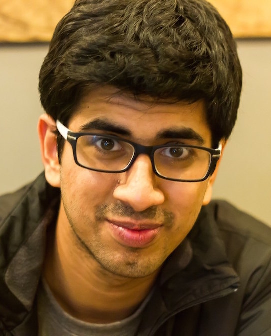
\includegraphics[width=1in,height=1.25in,clip,keepaspectratio]{figures/categoryshapes/shubham.pdf}}]{Shubham Tulsiani}
% received the B.Tech degree in Computer Science and Engineering from Indian Institute of Technology, Kanpur in 2013. He is currently a graduate student with the EECS Department, University of California, Berkeley. His research interests lie at the intersection of recognition, pose estimation and reconstruction from a single image. He is a recipient of the Berkeley Graduate Fellowship, CVPR Best Student Paper Award and International Physics Olympiad Gold medal.
% \end{IEEEbiography}

% \begin{IEEEbiography}[{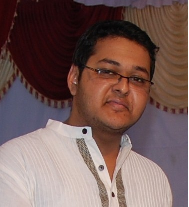
\includegraphics[width=1in,height=1.25in,clip,keepaspectratio]{figures/categoryshapes/akar.pdf}}]{Abhishek Kar}
% is a fourth year PhD student at UC Berkeley advised by Prof. Jitendra Malik. He obtained his B.Tech degree in Computer Science and Engineering from Indian Institute of Technology, Kanpur in 2012 where he worked on problems in human computer interaction and intelligent tutoring systems and received the Honda Young Engineer and Scientist (YES) Award. His primary research interest lies in 3D reconstruction of objects and scenes in the wild by leveraging advances in object/scene recognition. He is a recipient of the CVPR Best Student Paper Award and the Outstanding GSI Award at UC Berkeley.
% \end{IEEEbiography}

% \begin{IEEEbiography}[{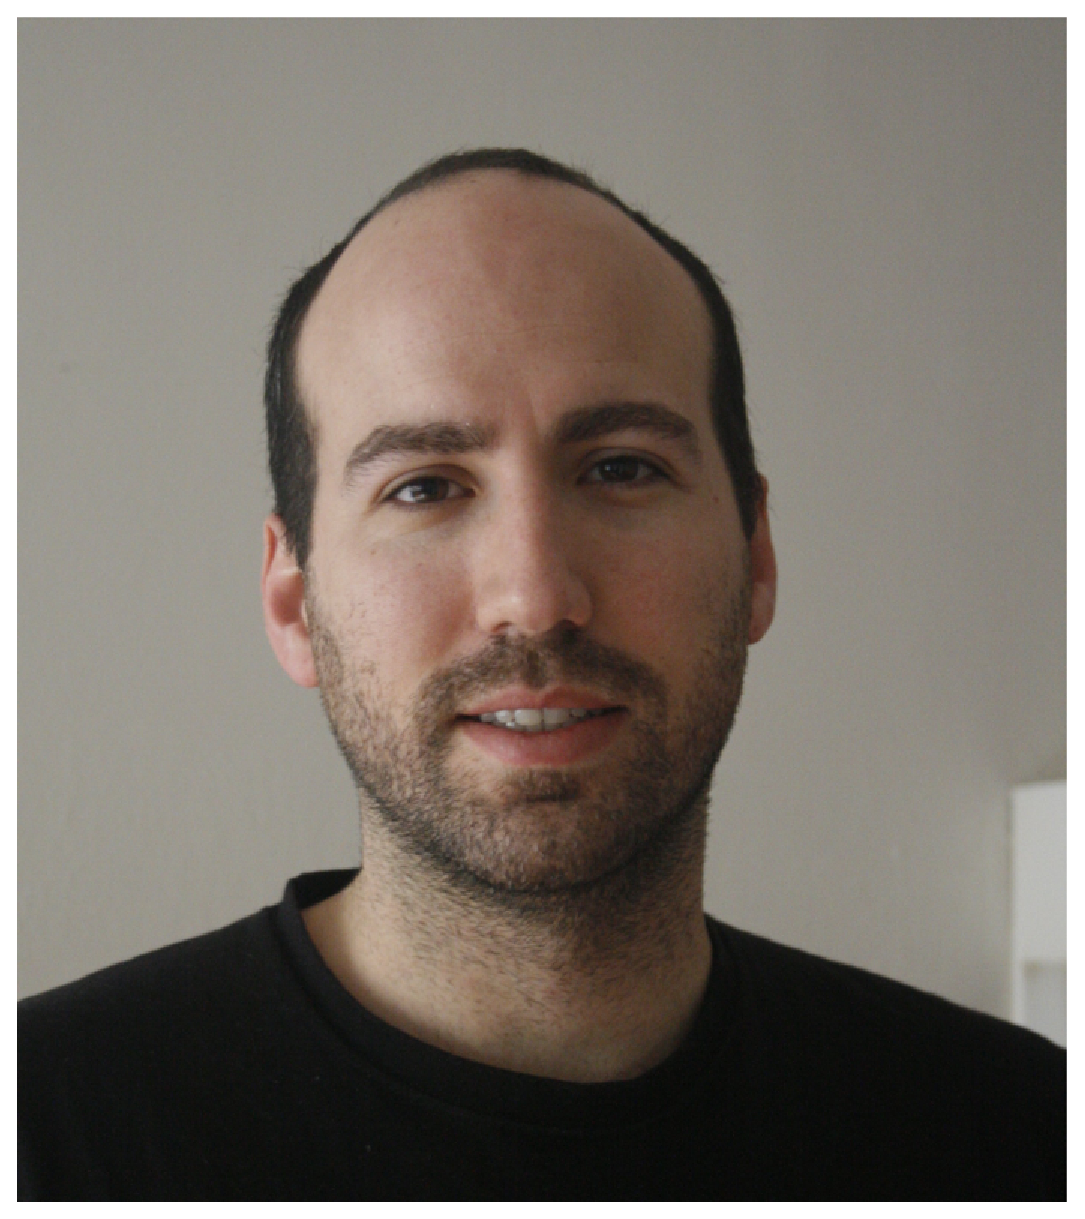
\includegraphics[width=1in,height=1.25in,clip,keepaspectratio]{figures/categoryshapes/joao.eps}}]{Jo\~{a}o Carreira}
% received his doctorate from the
% University of Bonn, Germany. His thesis focused
% on sampling class-independent object segmentation
% proposals using the CPMC algorithm, and
% on applying them in object recognition and localization.
% Systems authored by him and colleagues
% were winners of all four PASCAL VOC
% Segmentation challenges, 2009-2012. He did
% post-doctoral work at the Institute of Systems
% and Robotics in Coimbra, Portugal and is currently
% with the EECS department, at the University
% of California in Berkeley, USA. His research interests lie at the
% intersection of recognition, segmentation, pose estimation and shape
% reconstruction of objects from a single image.
% \end{IEEEbiography}

% \begin{IEEEbiography}[{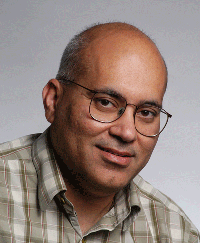
\includegraphics[width=1in,height=1.25in,clip,keepaspectratio]{figures/categoryshapes/jmalik.pdf}}]{Jitendra Malik}
%  is Arthur J. Chick Professor in the Department of Electrical Engineering and Computer Science at the University of California at Berkeley, where he also holds appointments in vision science, cognitive science and Bioengineering. He received the PhD degree in Computer Science from Stanford University in 1985 following which he joined UC Berkeley as a faculty member. He served as Chair of the Computer Science Division during 2002-2006, and of the Department of EECS during 2004-2006. Jitendra's group has worked on computer vision, computational modeling of biological vision, computer graphics and machine learning. Several well-known concepts and algorithms arose in this work, such as anisotropic diffusion, normalized cuts, high dynamic range imaging and shape contexts.  He was awarded the Longuet-Higgins Award for “A Contribution that has Stood the Test of Time” twice, in 2007 and 2008, received the PAMI Distinguished Researcher Award in computer vision in 2013 and the K.S. Fu prize in 2014. Jitendra Malik is a Fellow of the IEEE, ACM, and the American Academy of  Arts and Sciences,  and  a member of the National Academy of Sciences and the National Academy of Engineering.
% \end{IEEEbiography}
% \vfill

